\section{The Single-Particle Propagator}
The central project of the Dispersive Optical Model (like any optical model) is
to understand how nucleons move about in a nuclear many-body system. Specifically,
we wish to know
how a nucleon with energy $E$ and quantum numbers $\alpha$
at time $t_{0}$ will be measured at a
later time $t$ with quantum numbers $\beta$ after its interaction with the
nuclear environment, which is modeled with an optical potential. Given the
Hamiltonian that incorporates this interaction, the Schr\"odinger equation
relates the Hamiltonian to the time evolution of this state:

\begin{equation}
    i\hbar\frac{\partial}{\partial t}\ket{\alpha, t_{0};t} = H\ket{\alpha,
    t_{0}; t}
\end{equation}

where $\ket{\alpha, t_{0},t}$ is the state at time $t$, given an initial state
$\ket{\alpha, t_{0}}$. Simple substitution shows that this initial state
propagates in time according to:

\begin{equation}
    \ket{\alpha, t_{0}, t} = e^{-\frac{i}{\hbar}H(t-t_{0})}\ket{\alpha, t_{0}}
\end{equation}

Concretely, given initial position quantum numbers $\bm{r}$, the wavefunction
of a state $\psi(\bm{r},t)$ is the sum of the contributions of 

\begin{figure}
    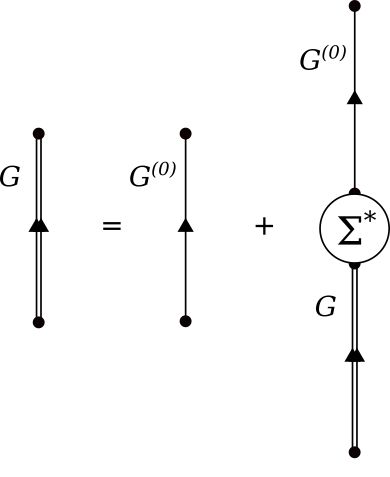
\includegraphics[scale=0.35]{figures/DysonEquation.png}
    \caption{The Dyson Equation in diagrammatic form}
    \label{DysonEquation}
\end{figure}

\section{Connection to Experimental Observables}
Subtracted dispersion relation.

\subsection{Elastic and inelastic nucleon scattering}
\subsection{Bound-state properties}

\section{Parameterization of the Potential}

To parameterize the DOM's optical potential, we rely on standard functional
forms common in nuclear theory calculations.

The real part of the potential is comprised of a Hartree-Fock component and
a spin-orbit component (plus a Coulomb term if the projectile is a proton).
The Hartree-Fock component $V_{HF}$ has two subcomponents:

\begin{equation}
    V_{HF}(r,r') = V_{vol}(r,r') + V_{WB}(r)
\end{equation}

The non-local Hartree-Fock volume term $V_{vol}(r,r')$, is defined as
a Woods-Saxon form coupled to a Gaussian non-locality:

\begin{equation}
    V_{vol}(r,r') =
    \dfrac{-V}{1+e^{(r-R)/a}}\cdot\dfrac{1}{\pi^{\frac{3}{2}}\beta^{3}}
    \exp{\frac{|r-r'|^{2}}{\beta^{2}}}
\end{equation}

where $V$, $R$, and $a$ are the depth, radius, and diffuseness of the HF potential,
and $beta$ is the extent of the non-locality. The local Hartree-Fock wine-bottle
term $V_{wb}(r)$, named for resemblence to the dimple at the bottom of a wine
bottle, is defined as a Gaussian centered at the nuclear origin:

\begin{equation}
    V_{wb}(r) = V\exp{\frac{r^{2}}{\sigma^{2}}}
\end{equation}

The real spin-orbit component $V_{so}$
is defined using a derivative-Woods-Saxon shape to
accommodate the expectation that the spin-orbit coupling is strongest near the
nuclear surface:

\begin{equation}
    V_{so}(r,r') =
    \frac{d}{dr} \frac{-V}{1+e^{\frac{(r-R)}{a}}}\cdot\frac{1}{\pi^{\frac{3}{2}}\beta^{3}} \exp{\frac{|r-r'|^{2}}{\beta^{2}}}
\end{equation}

The imaginary part of the potential is comprised of independent surface and volume terms
both above and below the Fermi surface, plus an imaginary spin-orbit term:

\begin{equation}
    V_{HF}(r,r') = V_{vol}(r,r') + V_{WB}(r)
\end{equation}

The occupation number of nucleons with quantum numbers $\alpha$ can be
calculated directly from the imaginary component of the single-particle
propagator:

\begin{eqnarray}
    n(\alpha)
    & = & \braket{\Psi^{N}_{0}|a^{\dagger}_{\alpha}a_{\alpha}|\Psi^{N}_{0}}\\
    & = & \sum_{n}|\braket{\Psi^{N-1}_{n}|a_{\alpha}|\Psi^{N}_{0}}|^{2}\\
    & = & \int_{-\infty}^{\epsilon_{F}^{-}} dE
\sum_{n}|\braket{\Psi^{N-1}_{n}|a_{\alpha}|\Psi^{N}_{0}}|^{2}
\delta(E-(E^{N}_{0}-E^{N-1}_{n}))\\
& = & \int_{-\infty}^{\epsilon_{F}^{-}} dE \frac{1}{\pi}\operatorname{Im}G(\alpha,\alpha;E)
\end{eqnarray}


For nuclei with open subshells (e.g., the $\upnu$ 0\dFive in $^{18}$O and
$\upnu$ 0\fFive in $^{58}$Ni), an additional
pairing parameter $\Delta$ was added to
account for these subshells' fractional occupatio $n_{\pm}$ of the open subshells. due to pairing
effects. This parameter splits partially-occupied subshells (e.g., the $\upnu$\dFive
for \oEight) into upper and lower sublevels with energies $E_{\pm}$:

\begin{equation}
    E_{\pm} = \mu \pm ((\epsilon_{F}-\mu)^{2} + \Delta^{2})^{frac{1}{2}}
\end{equation}

where $\mu$ is the energy of the open subshell before pairing is considered and
$\epsilon_{F}$ is the Fermi
energy. The magnitude of $\Delta$ corresponds to the energy difference between
adding/removing a nucleon to/from that subshell. The subshell's particle
capacity is split between the upper and lower sublevels, and only the :

\begin{equation}
    n_{\pm} = \frac{1}{2}\left( 1-\frac{\chi}{E_{\pm}}\right)
\end{equation}

where $\chi = |E_{\pm}-\mu| - (\epsilon_{F} - \mu)$. Only occupation in the
lower sublevel is counted toward the total particle number. For each open-shell
nucleus with nucleon numbers $N, Z$ , the pairing gap $\Delta$ was fixed according to:

\begin{equation}
    \Delta(N,Z) = \frac{1}{4}\left(B(N-2,Z)-3B(N-1,Z) + 3B(N,Z)-B(N+1,Z)\right)
\end{equation}

where $B(N,Z)$ is the nuclear binding energy.

The Dispersive Optical Model (DOM) is a phenomenological framework useful for 
extracting information about nuclear properties and structure from experimental
data.

The fundamental object of interest in the DOM is the \Gls{optical potential},
which is identified as the \Gls{nucleon self-energy}. This potential represents
the nuclear environment experienced
by a nucleon as it traverses the nucleus being represented. In general, the
potential is both non-local and complex, possessing both real (flux-conserving)
and imaginary (flux-removing) parts. The functions used to parameterize the optical potential
are selected to conform with general physical intuition about the nuclear
many-body problem and past experience with optical potentials throughout the
field. For example, the most important term, the Hartree-Fock (HF) potential
that binds the nucleus together, is defined by a classic Woods-Saxon form to
which non-locality has been added: [insert volume term formula]. The imaginary
potential is separated into a Woods-Saxon volume component and a
Woods-Saxon-derivative surface component. Each of these subcomponents has
a non-linear energy dependence reflecting our expectation that surface-like
behaviors should arise around 10-20 MeV and volume-like behavior should dominate
above 50 MeV, with a mixture of the two in the intermediate region.

Beyond these basic considerations, several additional features make the 
DOM a useful tool. First is the enforcement of a
dispersion relation (the Kramers-Kronig relations) between the real and imaginary
halves of the potential, ensuring that the potential is causal (i.e., the
time-ordering of the operator representation of the self-energy is maintained).

\section{Computational Improvements}
As with any high-dimensional optimization problem, the fitter must be vigilant
against the overfitting of data. In practice, this requires:

parsimony with the number of parameters used in the model

common-sense checking "under the hood" of the optimization to verify that
parameter values make sense given the assumptions that undergird the model

understanding of what the value function is (that is, the function being
minimized/maximized) and whether it needs to be changed

cross-correlation between parameters to understand the relationship between
parameters and the effect that each has on predictions made using the model

TCS affected by HF parameters, spin orbit, imaginary above
RCS affected by imaginary above, HF parameters
ECS affected by HF parameters, spin orbit, imaginary above
APower affected by HF parameters, spin orbit,  imaginary above
Charge Density affected by HF parameters, imaginary below
Levels affected by HF parameters, spin orbit,
Spectral functions affected by HF parameters, imaginary below
RMSRadii affected by HF parameters, imaginary below

Physical intuition about scattering data:
- the low-angle ECS/APower data are sensitive to the imaginary strength above
the Fermi surface. The high-angle ECS/APower data are sensitive to the imaginary
strength below the Fermi surface, with the highest angles of elastic scattering
probing the imaginary strength deepest in the core (see high-energy, high-angle
data in Pb)
- the NM correction to the imaginary volume strength is required in all cases to
have the very high/very low energy imaginary strength have the correct trend
(linearly increasing above 100 MeV above, decreasing to 0 below 100 MeV below).
Seen in spectral functions and total cross section data at high energies, where
the pion production channel enters the picture as it goes from virtual->real
- the general trend of the elastic scattering data (not wiggles, but averaged
over wiggles) depends on the imaginary strength at the given energy. If the
minima in the elastic cross sections are too sharp/deep, the imaginary strength
is too large at that energy
- the spin-orbit strength has dramatic effects on the total cross section at low
energies ($<$20 MeV)
- above the Fermi surface, the imaginary strength is dominated by surface from
0-50 MeV and by volume from 50 MeV up. Below the Fermi surface, the surface
imaginary strength is dependent on A; for low A, where the level density is very
low below the Fermi surface and there's almost no contribution from high LJ
levels, there is virtually no surface imaginary strength below (cf. with charge
density distribution tail, at the surface of the nucleus). As A increases, 
imaginary surface strength below increases gradually but never reaches the
imaginary surface strength above. A consequence of the asymmetry of the
operators that contribute: below 0 MeV, the removal operator LJs
must recouple to the ground state, so high LJ operators have virtually no
contribution; above 0 MeV, addition operators can have arbitrary LJs because
free scattering is possible, adding significantly to the collective strength and
thus is imaginary strength peaked at the surface in the 20-30 MeV range (giant
dipole resonance, for example, surface phonons).

\subsection{Fitting procedure}
The powell method, outlined in Numerical Recipes in C \cite{NumericalRecipes},
was used to minimize the RMS difference between experimental data points and the
values calculated by the DOM. A weighting scheme was assigned to the data points
according to their importance, guiding the fit to reproduce the most essential
data points. From fit to fit, the weighting scheme was adjusted as necessary to
escape local minima in the multidimensional fit.

The radial grid, energy grid, size of the lagrange basis, partial wave angular momentum cutoff, and
various integration cutoffs used in calculating the potential and
observable quantities were varied to ensure that output was not distorted by numerical errors. 

\subsection{Generalization to even-even nuclei}
- 

\afterpage{\clearpage}
